%\section{Terminology}
%\label{sec:term}

%The weight in the
%relation is used to measure the frequency of the relation in a large
%corpus. This weight can be used to calculate: 1) conditional probability
%of an entity given a concept (e.g., the probability of ``Microsoft''
%given the concept ``company'' is higher than that of ``Douban'' which is a
%website for sharing comments on books, movies or music); and 2)
%the conditional probability of a concept given an
%entity (e.g., the probability of ``fruit'' given ``apple'' is higher
%than that of ``plant'').

\section{Problem Definition}
\label{sec:problem}
We start with defining the problem of action 
conceptualization on each argument of the verb. Since 
verbs are often used together with more than one arguments, 
typically subject and object, 
conceptualising each argument may not be enough to understand
the usage of the verb. 
Thus, we further define the action conceptualization problem 
of subject-verb-object triplets to model the relations between subjects
and objects.

\subsection{Action Conceptualization}
We first define {\em taxonomy}.
%to guide the levels of abstraction when
%generalizing the arguments of verbs.
A taxonomy is a direct acyclic graph $(V, E)$.
Here, $V$ is a set of terms, $E$ is a set of binary ``isA'' relations
\[E=\{(e,c)| e\in V, c\in V, e~ isA~ c\},\]
where $e$ is called an {\em entity},
$c$ is called a {\em concept}, and $c$ is said to {\em cover} $e$.
%For example, if a taxonomy contains the following relations:
%``apple'' isA ``fruit'' and ``Barack Obama'' isA ``politician'',
%then ``apple'' and ``Barack Obama'' are entities while ``fruit''
%and ``politician'' are concepts. 
Most terms in $V$ are
both a concept and an entity; only those leaf nodes in the graph are
entities only. We use the taxonomy to guide the levels of
abstraction when generalizing the argument of verbs in the following
problem.

We begin with an informal definition of the
{\em action conceptualization} problem.
Given a collection of argument instances of the same argument
type (e.g., object or subject) of a
verb, %which are extracted from a text corpus,
we want to pick $k$ concepts from the taxonomy
that cover as many instances as possible, which
is equivalent to maximizing the likelihood of the corpus.
%That is, for each argument instance,
%there must be at least one concept in $O$ which subsumes the argument
%in an isA relation.
%A {\em concept} is defined as any {\em non-leaf} node
%in the taxonomy.
On the other hand, we would like these $k$ concepts to
have little overlap against each other.
%The intuition is that the $k$ concepts thus selected independently
%represent a unique semantic use but collectively cover majority of the uses
%of that verb.
The intuition is that each of the $k$ selected concepts represents a unique
semantic and the $k$ concepts collectively cover majority of the 
uses of that verb.
%the selected k concepts to be as small as possible
%so each of these concepts essentially
%represent a different use of the verb.
%The resulting action concepts are similar to the definition entries of
%words in a dictionary.
For example, for verb ``wear'', the list of extracted
object argument instances might be ``t-shirt'', ``hoodie'', ``stetson hat'', ``bracelet'',
``ear ring'', ``pink'', etc. One way of conceptualizing the objects of
``wear'' might be ``clothing'', ``accessory'' and ``style'', which arguably
describe different meanings of ``wear''.
\KQ{This example may need to change.}

%Notice that the only criteria for us to choose these $k$ concepts are their
%coverage of the argument instances and the overlaps. The additional entities
%covered by a concept but {\em not} in set of argument instances
%are not of concern.
%This is because the key purpose of an action concept is to provide an
%abstraction for a class of arguments, even those that were never seen before
%in the data.
%We rely on a taxonomy to provide such isA relations.
%Probase is a large scale of IsA knowledge base derived from
%large collection of web pages.
%It contains information about relation between concept and entity
%which entity is an instance of concept and the probability of that relation.
%If we view each concept in Probase as a set of entities,
%the target of our problem is to pick a list of concepts in Probase
%which the union of these concepts contains all the objects in the
%given collection so those concepts can cover the usage of the verb.
%For example, given objects ``shoe'', ``hat'', ``shirt'',
%``red'' and ``yellow'' for verb ``wear'', we may obtain the
%following concepts, which ``clothing'' covers ``shoe'', ``hat'' and
%``shirt" while ``color" covers ``red'' and ``yellow.''
%``Clothing'' and ``color'' represent the different usages of ``wear.''
%
%\KZ{First define the problem informally, and then go into the
%mathematical definition.}
%We first define the problem of \emph{action conceptualization} informally.
%
%\KZ{Do not refer to Probase here, but instead define the problem
%purely on set of entities.}
%We want to find a set of
%concepts which can cover all the objects extracted from the corpus,
%that is, for each object, we can at least find one concept in the set having
%IsA relation with that object. During the extraction, we just keep those
%objects that can be mapped to entities. If we view each Probase
%concept as a set of entities, our process is similar to the classical set
%cover problem. All the objects extracted from the entities set $U$ to be
%covered, Probase itself is a set $S$ of entities set so the problem is to
%identify a smallest subset of $S$ whose union contains all the entities in $U$.
%The Difference is that, in our problem, the union of sets in $S$ may be
%larger than $U$, while in the classical set cover problem, $U$ and the union
%of sets in $S$ is equal. Formally, our problem can be formulated as follow:
The above intuition leads to the following formal definitions.
\begin{definition}
\emph{Overlap}:
The overlap between two concepts is
\begin{equation}
\label{eq:overlap}
Overlap(c_1,c_2)=\frac{|E_{c_1}\cap E_{c_2}|}{min\{ |E_{c_1}|,|E_{c_2}| \}},
\end{equation}
where $E_c$ is the set of all entities covered by concept $c$ in the
taxonomy.
\end{definition}
Next, we define \emph{concept graph}, which is a graph of concepts
with bounded pairwise overlaps.
Let $C$ be the collection of all concepts in the taxonomy,
where each concept $c$ covers a set of entities $E_c$.
\begin{definition}
\emph{Concept Graph}: A concept graph is an
undirected graph $G=(C,L)$, where
$C$ is the set of concepts and $L$ is the set of edges between
two concepts. An edge $l_{c_1,c_2}\in L$ between $c_1$ and $c_2$ exists iff
$Overlap(c_1, c_2)\leq\tau$, where $\tau$ is a threshold.
\end{definition}

\figref{fig:graph_model} shows 4 concepts in an illustrative 2-dimensional
entity space (a), as well as their corresponding concept graph (b).
Each circle $c_i$ in (a) represent a set of entities covered by concept $c_i$.
Because there is heavy overlapping ($>\tau$) in entities between $c_0$ and $c_3$
and between $c_1$ and $c_3$, (b) is a fully connected graph (clique) minus only
two edges: $l_{c_0,c_3}$ and $l_{c_1, c_3}$.
%Assume that we have 7 concepts in the taxonomy,
%and the corresponding concept graph is (a).
%Taking concepts $c_0$ to $c_3$ for illustration, $c_0$ is connected with $c_1$, while not connected with $c_3$.
%Because the overlap of $c_0$ and $c_1$ is small enough to satisfy the threshold while the overlap of
%$c_0$ and $c_3$ is not, as we can see from (b). The circle of a concept $c$ represents for its entity
%set $E_c$ in the taxonomy.

\begin{figure}[th]
\centering
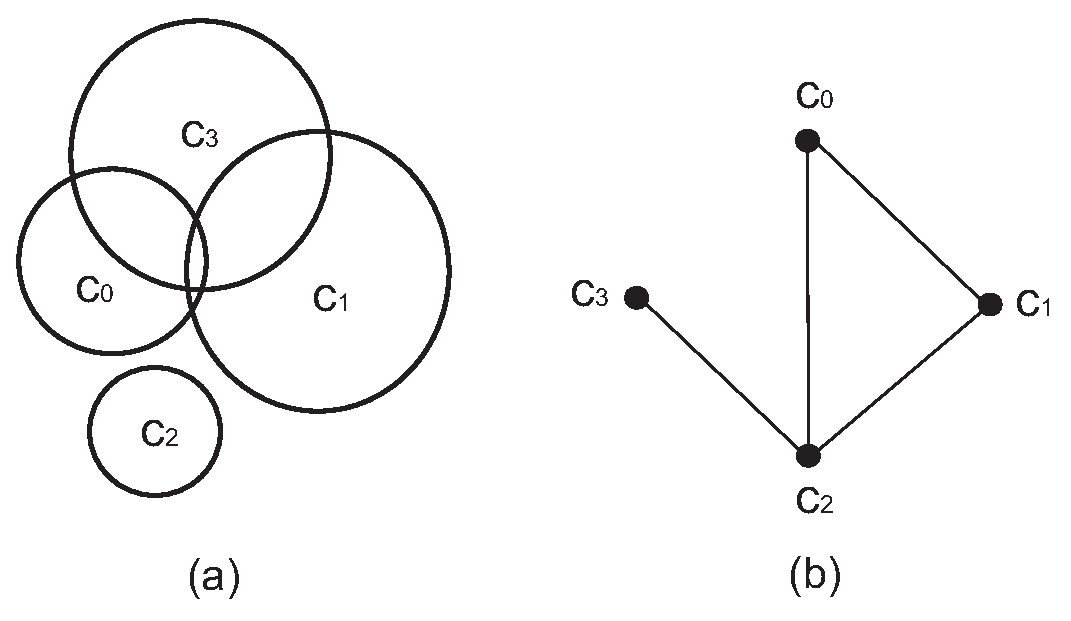
\epsfig{file=figure/graph_model.eps,width=0.6\columnwidth}
\caption{(a) Illustration of 4 Concepts in the Entity Space
(b)The Corresponding Concept Graph
}
\label{fig:graph_model}
\end{figure}

Considering that the argument instances may have different 
importances to the verb in common sense, e.g., ``eat food'' is more common than ``eat word'',
we use $Q_v(e)$ to define the quality of argument instance $e$ in $A_v$ w.r.t.
a verb $v$. On the other hand, concepts may be different in the quality of 
summarizing the arguments. For example, vague concepts like ``word'' may be 
able to cover most of the arguments in $A_v$, but there are too many 
entities not appeared in $A_v$. We use $Q_v(c)$ to denote the 
quality of a concept if it's used to abstract the argument of verb $v$.
Then, we formulate the action conceptualization problem as:
\begin{definition}
\emph{Action Conceptualization}: 
Given a concept graph $G=(C,L)$,
the set of entities $E_c$ for each concept $c\in C$,
and a set of argument instances $A_v$ for a verb $v$, find a clique
with $k$ nodes $C_k\subseteq C$
in $G$ that maximizes the following function:
\begin{equation}
\begin{split}
f_v(C_k)&=\sum_{e\in A_v}{\sum_{c\in C_e\cap C_k}{Q_v(e)Q_v(c)Pr(c|e)}} \\
&=\sum_{c\in C_e\cap C_k}{Q_v(c)\sum_{e\in A_v}{Q_v(e)Pr(c|e)}}
\end{split}
\label{eq:objective}
\end{equation}
\end{definition}

Here is an intuitive explanation for \eqnref{eq:objective}. 
Since each argument $e$  of verb $v$ may be covered by a number of concepts, 
the quality mass $Q_v(e)$ is distributed by the probability $Pr(c|e)$ to 
all concepts that cover $e$. The objective of the problem is to select 
$k$ concepts with largest total distributed quality mass, weighted by the 
quality of these concept.

\subsection{Action Conceptualization on Triplets}
%Beyond the definition of the action conceptualization problem 
%on each argument of a verb, we define the problem of conceptualizing 
%subject-verb-object triplets. 
We first define the concept graph on
triplets:
\begin{definition}
\emph{Triplet Concept Graph}: A concept graph is an
undirected graph $G'=(P,L')$, where
$P$ is the set of pairs of concepts and $L'$ is the set of edges between
two pairs. Each pair of concepts is denoted by $p=\{c_s, c_o\}$.
An edge $l_{p_1,p_2}\in L'$ between $p_1$ and $p_2$ exists iff
\begin{equation}
\begin{split}
\min{}&(Overlap(p_1.c_s, p_2.c_s), \\
&Overlap(p_1.c_o, p_2.c_o))\leq\tau,\\
\end{split}
\end{equation}
where $\tau$ is a threshold.
\end{definition}
The definition of triplet concept graph constrains that at least one of the two 
concepts in the concept pair satisfies the overlap constraint. For example, 
``person eat food'' and ``person eat word'' are two different usages of eat.
Although subject concepts are the same, there is still
an edge between \{``person'',``food''\} and \{''person'', ``word''\}, because the 
objects satisfiy the overlap constraint.

We now define action conceptualization on triplets on the triplet concept 
graph. Similar to the definition for each argument, we want to find out 
$k$ concept pairs in the triplet concept graph that maximize the quality 
mass on both subject and object.
We denote a triplet instance as $\{e_s, v,  e_o\}$, i.e., the subject, verb and 
the object.
%And we use $f_{s-v}(C_k)$ to denote the 
%scoring function in \eqnref{eq:objective} on the subject side, and $f_{v-o}(C_k)$ 
%to denote the scoring function on the object side. 
The action conceptualization problem on triplets is:
\begin{definition}
\emph{Action Conceptualization}: 
Given the triplet concept graph $G'=(P,L')$, 
the set of entities $E_c$ for each concept $c\in C$,
and a set of triplet instances $T_v$ for a verb $v$, find a clique
with $k$ nodes $P_k\subseteq P$
in $G'$ that maximizes the following function:
\begin{equation}
\begin{split}
f_v(P_k)&=\sum_{p\in P_k}{f_{v,s}(p.c_s)\times f_{v,o}(p.c_o)}\\
f_{v,s}(c)&=Q_{v,s}(c)\sum_{e\in A_{v,s}}{Q_{v,s}(e)P(c|e)} \\
f_{v,o}(c)&=Q_{v,o}(c)\sum_{e\in A_{v,o}}{Q_{v,o}(e)P(c|e)}.
\end{split}
\label{eq:objectivetri}
\end{equation}
\end{definition}
In \eqnref{eq:objectivetri}, $A_{v,s}$ is the subject set of verb $v$, and $Q_{v,s}(c)$ is
the quality of concept $c$ as the subject of the verb, and $Q_{v,s}(e)$ is
the quality of entity $e$ as the subject of the verb. Notations 
$A_{v,o}$,$Q_{v,o}(c)$ and $Q_{v,o}(e)$ are defined similarly for the 
object of the verb.

%The action conceptualization can thus be formulated as a
%modified $k$-clique problem:
%\begin{definition}
%\emph{Action Conceptualization}: 
%Given a concept graph $G=(C,L)$,
%the set of entities $E_c$ for each concept $c\in C$,
%and a set of argument instances $A_v$ for verb $v$,
%find a clique with $k$ nodes $C_k\subseteq C$
%in $G$ that maximizes a submodular function
%\begin{equation}
%f(C_k)=|\bigcup_{c\in C_k}{E_c}\cap A_v|.
%\end{equation}
%\end{definition}
%
%The above definition assumes that every element of $A_v$ is a correct argument
%of $v$ and should be covered by $C_k$.
%However, in practice, argument instances extracted from large text corpus
%using parsers may contain errors. In order to handle such noise,
%we generalize the problem to incorporate a \emph{confidence score} $g_v(e)$
%of each entity $e$ under verb $v$:
%%Suppose we have a way to measure the confidence of whether the
%%argument instance is right for the verb $v$,
%%we define that measure as a function $g_v(e)$.
%%The generalized action conceptualization problem is thus:
%\begin{definition}
%\label{def:acw}
%\emph{Generalized Action Conceptualization}:
%Given a concept graph $G=(C,L)$,
%the set of entities $E_c$ for each concept $c\in C$,
%and a set of argument instances $A_v$ for a verb $v$, find a clique
%with $k$ nodes $C_k\subseteq C$
%in $G$ that maximizes a weighted submodular function
%\begin{equation}
%f(C_k)=\sum_{e\in \bigcup_{c\in C_k}{E_c}\cap A_v}{g_v(e)}.
%\label{eq:f}
%\end{equation}
%\end{definition}

%\KQ{
%\begin{equation}
%\begin{split}
%f(C_k)&=\sum_{e\in A_v}{\sum_{c\in C_e\cap C_k}{Q(e)Q(c)P(c|e)}} \\
%&=\sum_{c\in C_e\cap C_k}{Q(c)\sum_{e\in A_v}{Q(e)P(c|e)}}
%\end{split}
%\end{equation}
%\begin{equation}
%\begin{split}
%Q(e)=-\sum_{m\in M_{e,v}}{P(m)\log{P(m)}} \times MI(e), \\
%Q(c)=\frac{1}{1+\sum_{e\in A_v\cup E_c}{P(e|c)\log{\frac{P(e|c)}{P(e|A_v)}}}},
%\end{split}
%\end{equation}
%where $m$ is a syntactic pattern from which we extracted $e$ as the 
%argument of the verb $v$. $Q(c)$ is the KL-divergence between $P(e|c)$
%and $P(e|A_v)$, When either of the probability equals to 0, the KL-divergence
%equals to 0.
%}
%To define the confidence function $g_v$ for a verb $v$,
%we suppose that the arguments related to the verb contain more
%information than the ones that are not related to that verb. For example, ``basketball''
%is a informative object of the verb ``play'', while ``weekend'' less informative to ``play''.
%Since ``basketball'' appears many times in the context of the ``play'', but does not appear
%in the context of many other verbs. However, ``weekend'' can appear in the context of many
%verbs according to the wrong parsing (e.g., recognized as the object of ``play'', ``go'', ``buy'',
%etc.).
%Mutual information is a measure in information theory which can capture this information. In
%this paper, we use binary version of the mutual information to define function $g_v$:
%\begin{eqnarray}
%\min && \sum_{s\in S} x_s \\
%\rm{subject~to} && \sum_{s:e\in s} x_s \ge 1,\ \forall e \in U \label{eq:cover}\\
%&& x_s\in \{0,1\},\ \forall s \in S \label{eq:binary} \\
%% && \frac{|s\cap U|}{|s|} \ge 0.9\ for\ all\ s:x_s=1 \\
%% && \sum_{s,t:x_s=1,x_t=1} |s\cap t| \le \tau
%&& \frac{|s\cap t|}{min\{ |s|,|t| \}} \le \tau,\ \mbox{for~}  x_s=1, x_t=1
%\label{eq:overlap}
%\end{eqnarray}
% If $\bigcup_{s\in S}s = U$, then $|s\cap U| = |s|$, constraint (4) is always satisfied so we can remove it.
%\textcolor{red}{
%\begin{eqnarray}
%\min_{\tau,t, x} && \tau, t \\
%\rm{subject~to} && x_s(x_s-1)=0 \label{eq:zo}\\%\in [0,1],\ \forall s \in S \\
%&&\sum_{s\in S}{x_s}=k \label{eq:k}\\
%&& x^TPx \le \tau \label{eq:cover}\\
%%&&-\sum_{e\in U}{\sum_{s:e\in V_s}{x_s{A(p,s)}}} \le t
%%&&-\sum_{s\in S}{x_s \sum_{e\in U\cap V_s}{I(p,e)}} \le t
%&& -d^Tx \le t
%\end{eqnarray}
%\begin{eqnarray*}
%\max_{x} && \sum_{s\in S}{Coverage(s)\cdot x_s} \\
%\rm{subject~to} && x_s\cdot (x_s-1)=0\\
%&&\sum_{s\in S}{x_s}=k\\
%&& Overlap(s,t)\cdot x_t\cdot x_s\leq \tau, for\ all\ s,t\in S, s\neq t
%\end{eqnarray*}
%where $x=\{x_s|s\in S\}$ is a decision vector (each dimension is either 0 or 1) illustrating that whether a concept $s$ in candidate concept set $S$ is chosen or not.
%Matrix $P$ is the overlap matrix storing the pairwise concept overlap which is a constant to the problem. And the overlap score between concept $s$ and $t$ is formulated as follow.
%$$
%Overlap(s,t)=\frac{|V_s\cap V_t|}{min\{ |V_s|,|V_t| \}}
%$$
%where $V_s$, $V_t$ are the entity set of the concept $s$ and $t$.
%Vector $d$ is the coverage vector storing each concept coverage which is also a constant to the problem. And the coverage score of concept $s$ is formulated as follow.
%$$
%Coverage(s)=\sum_{e\in U\cap V_s}{BMI(v,e)}
%$$
%where $U$ is set of all extracted argument instances of a verb $v$ and $BMI(v,e)$ represents Binary Mutual Information of the verb $v$ and the argument instance $e$ which is formulated as follow.
%$$
%g_v(e)=
%\begin{cases}
%1 & if\ p(v,e)\log \frac{p(v,e)}{p(v)p(e)}> 0\\
%-1 & otherwise
%\end{cases}
%$$
%The probability $p(v,e)$ is the co-occurrence probability
%of $v$ and $e$ in corpus, $p(v)$ and $p(e)$ are
%the occurrence probability of $v$ and $e$ in corpus.
%, where $V_s$ is the entity set of the concept $s$,
%and $X=\{x_s|s\in S\}$ is an indicating vector (each dimension indicates the selection of a concept).
%Function $I(p,s)$ is the mutual information between predicate $p$ and class $s$.
%It is defined as follows:
%\begin{equation}
%I(p,s)=\sum_p{p(p)\sum_s{p(s|p)log\frac{p(s|p)}{p(s)}}}
%\end{equation}
%Matrix $P$ is the overlap matrix stores the pairwise concept overlap which is a constant to
%the problem.
%If this matrix is positive semi-definite,
%the problem is convex.
%The problem can be viewed as a multi-objective QCQP
%(Quadratically Constrained Quadratic Program).
%Usually, the diagonal elements are all positive and
%larger than or equal to all other elements, it is possibly be positive semi-definite. Even though
%it is not positive semi-definite, we can enlarge elements in the diagonal to construct a positive
%semi-definite version. Because we do not care the diagonal in the problem but other elements, we
%can modify the diagonal without affecting the solution of $X$.
%}

%The problem is a maximum weighted k-clique finding problem.
%Because the k-clique finding problem, a special case of
%the weighted version (all weights are 1), is NP-hard, the action
%conceptualization problem is also NP-hard.
%
%\begin{lemma}
%Action conceptualization (AC) problem and generalized action
%conceptualization (GAC) problem are NP-hard.
%\end{lemma}
%\begin{proof}
%AC is a special case of GAC.
%A special case of AC is when each concept in the graph
%contains exactly one distinct entity which is also in $A_v$.
%As such, the submodular function is simplified to $f(C_k) = |C_k|$.
%The problem is then reduced to finding all k-cliques in the graph,
%which is a known NP-hard problem\cite{Vassilevska2009254}.
%Thus, AC is NP-hard and GAC is also NP-hard.
%%\qed
%\end{proof}
%
%In following, we refer to GAC as AC for simplicity.
